
\section{Vullen van vierkanten en kubussen}

\subsection{Vierkant vullen met vierkanten}

In hetgeen komt zullen we steeds met natuurlijke getallen werken. We zullen voor geen enkele grootte een kommagetal of een breuk nemen. Nemen we een vierkant met zijde $10$, dan kan dit vierkant gevuld worden met $100$ kleinere vierkantjes van grootte $1$. Dit is duidelijk in Figuur \ref{fig:vierkant10_1x1}. Hetzelfde vierkant kunnen we ook vullen met vierkantjes van grootte $2$, waarbij we nu $25$ kleinere vierkantjes hebben in het grote vierkant. Als we nu echter dit vierkant compleet wensen te vullen met vierkantjes van grootte $3$, dan zien we dat dit niet lukt, zie Figuur \ref{fig:vierkant10_3x3}.

\begin{figure}[ht]
  \centering
  \subfloat[in vierkantjes met zijde $1$]{\label{fig:vierkant10_1x1}\definecolor{cqcqcq}{rgb}{0.75,0.75,0.75}
\begin{tikzpicture}[scale=0.45,line cap=round,line join=round,>=triangle 45,x=1.0cm,y=1.0cm]
\draw [color=cqcqcq,dash pattern=on 2pt off 2pt, xstep=1.0cm,ystep=1.0cm] (-0.5,-0.5) grid (10.5,10.5);
\clip(-0.5,-0.5) rectangle (10.5,10.5);
\filldraw[line width=1.6pt,fill=black,fill opacity=0.1] (0,0) -- (10,0) -- (10,10) -- (0,10) -- cycle;
\filldraw[fill=black,fill opacity=0.1] (0,0) -- (1,0) -- (1,1) -- (0,1) -- cycle;
\filldraw[fill=black,fill opacity=0.1] (1,0) -- (2,0) -- (2,1) -- (1,1) -- cycle;
\filldraw[fill=black,fill opacity=0.1] (2,0) -- (3,0) -- (3,1) -- (2,1) -- cycle;
\filldraw[fill=black,fill opacity=0.1] (3,0) -- (4,0) -- (4,1) -- (3,1) -- cycle;
\filldraw[fill=black,fill opacity=0.1] (4,0) -- (5,0) -- (5,1) -- (4,1) -- cycle;
\filldraw[fill=black,fill opacity=0.1] (5,0) -- (6,0) -- (6,1) -- (5,1) -- cycle;
\filldraw[fill=black,fill opacity=0.1] (6,0) -- (7,0) -- (7,1) -- (6,1) -- cycle;
\filldraw[fill=black,fill opacity=0.1] (7,0) -- (8,0) -- (8,1) -- (7,1) -- cycle;
\filldraw[fill=black,fill opacity=0.1] (8,0) -- (9,0) -- (9,1) -- (8,1) -- cycle;
\filldraw[fill=black,fill opacity=0.1] (9,0) -- (10,0) -- (10,1) -- (9,1) -- cycle;
\filldraw[fill=black,fill opacity=0.1] (0,1) -- (1,1) -- (1,2) -- (0,2) -- cycle;
\filldraw[fill=black,fill opacity=0.1] (1,1) -- (2,1) -- (2,2) -- (1,2) -- cycle;
\filldraw[fill=black,fill opacity=0.1] (2,1) -- (3,1) -- (3,2) -- (2,2) -- cycle;
\filldraw[fill=black,fill opacity=0.1] (3,1) -- (4,1) -- (4,2) -- (3,2) -- cycle;
\filldraw[fill=black,fill opacity=0.1] (4,1) -- (5,1) -- (5,2) -- (4,2) -- cycle;
\filldraw[fill=black,fill opacity=0.1] (5,1) -- (6,1) -- (6,2) -- (5,2) -- cycle;
\filldraw[fill=black,fill opacity=0.1] (6,1) -- (7,1) -- (7,2) -- (6,2) -- cycle;
\filldraw[fill=black,fill opacity=0.1] (7,1) -- (8,1) -- (8,2) -- (7,2) -- cycle;
\filldraw[fill=black,fill opacity=0.1] (8,1) -- (9,1) -- (9,2) -- (8,2) -- cycle;
\filldraw[fill=black,fill opacity=0.1] (9,1) -- (10,1) -- (10,2) -- (9,2) -- cycle;
\filldraw[fill=black,fill opacity=0.1] (0,2) -- (1,2) -- (1,3) -- (0,3) -- cycle;
\filldraw[fill=black,fill opacity=0.1] (1,2) -- (2,2) -- (2,3) -- (1,3) -- cycle;
\filldraw[fill=black,fill opacity=0.1] (2,2) -- (3,2) -- (3,3) -- (2,3) -- cycle;
\filldraw[fill=black,fill opacity=0.1] (3,2) -- (4,2) -- (4,3) -- (3,3) -- cycle;
\filldraw[fill=black,fill opacity=0.1] (4,2) -- (5,2) -- (5,3) -- (4,3) -- cycle;
\filldraw[fill=black,fill opacity=0.1] (5,2) -- (6,2) -- (6,3) -- (5,3) -- cycle;
\filldraw[fill=black,fill opacity=0.1] (6,2) -- (7,2) -- (7,3) -- (6,3) -- cycle;
\filldraw[fill=black,fill opacity=0.1] (7,2) -- (8,2) -- (8,3) -- (7,3) -- cycle;
\filldraw[fill=black,fill opacity=0.1] (8,2) -- (9,2) -- (9,3) -- (8,3) -- cycle;
\filldraw[fill=black,fill opacity=0.1] (9,2) -- (10,2) -- (10,3) -- (9,3) -- cycle;
\filldraw[fill=black,fill opacity=0.1] (0,3) -- (1,3) -- (1,4) -- (0,4) -- cycle;
\filldraw[fill=black,fill opacity=0.1] (1,3) -- (2,3) -- (2,4) -- (1,4) -- cycle;
\filldraw[fill=black,fill opacity=0.1] (2,3) -- (3,3) -- (3,4) -- (2,4) -- cycle;
\filldraw[fill=black,fill opacity=0.1] (3,3) -- (4,3) -- (4,4) -- (3,4) -- cycle;
\filldraw[fill=black,fill opacity=0.1] (4,3) -- (5,3) -- (5,4) -- (4,4) -- cycle;
\filldraw[fill=black,fill opacity=0.1] (5,3) -- (6,3) -- (6,4) -- (5,4) -- cycle;
\filldraw[fill=black,fill opacity=0.1] (6,3) -- (7,3) -- (7,4) -- (6,4) -- cycle;
\filldraw[fill=black,fill opacity=0.1] (7,3) -- (8,3) -- (8,4) -- (7,4) -- cycle;
\filldraw[fill=black,fill opacity=0.1] (8,3) -- (9,3) -- (9,4) -- (8,4) -- cycle;
\filldraw[fill=black,fill opacity=0.1] (9,3) -- (10,3) -- (10,4) -- (9,4) -- cycle;
\filldraw[fill=black,fill opacity=0.1] (0,4) -- (1,4) -- (1,5) -- (0,5) -- cycle;
\filldraw[fill=black,fill opacity=0.1] (1,4) -- (2,4) -- (2,5) -- (1,5) -- cycle;
\filldraw[fill=black,fill opacity=0.1] (2,4) -- (3,4) -- (3,5) -- (2,5) -- cycle;
\filldraw[fill=black,fill opacity=0.1] (3,4) -- (4,4) -- (4,5) -- (3,5) -- cycle;
\filldraw[fill=black,fill opacity=0.1] (4,4) -- (5,4) -- (5,5) -- (4,5) -- cycle;
\filldraw[fill=black,fill opacity=0.1] (5,4) -- (6,4) -- (6,5) -- (5,5) -- cycle;
\filldraw[fill=black,fill opacity=0.1] (6,4) -- (7,4) -- (7,5) -- (6,5) -- cycle;
\filldraw[fill=black,fill opacity=0.1] (7,4) -- (8,4) -- (8,5) -- (7,5) -- cycle;
\filldraw[fill=black,fill opacity=0.1] (8,4) -- (9,4) -- (9,5) -- (8,5) -- cycle;
\filldraw[fill=black,fill opacity=0.1] (9,4) -- (10,4) -- (10,5) -- (9,5) -- cycle;
\filldraw[fill=black,fill opacity=0.1] (0,5) -- (1,5) -- (1,6) -- (0,6) -- cycle;
\filldraw[fill=black,fill opacity=0.1] (1,5) -- (2,5) -- (2,6) -- (1,6) -- cycle;
\filldraw[fill=black,fill opacity=0.1] (2,5) -- (3,5) -- (3,6) -- (2,6) -- cycle;
\filldraw[fill=black,fill opacity=0.1] (3,5) -- (4,5) -- (4,6) -- (3,6) -- cycle;
\filldraw[fill=black,fill opacity=0.1] (4,5) -- (5,5) -- (5,6) -- (4,6) -- cycle;
\filldraw[fill=black,fill opacity=0.1] (5,5) -- (6,5) -- (6,6) -- (5,6) -- cycle;
\filldraw[fill=black,fill opacity=0.1] (6,5) -- (7,5) -- (7,6) -- (6,6) -- cycle;
\filldraw[fill=black,fill opacity=0.1] (7,5) -- (8,5) -- (8,6) -- (7,6) -- cycle;
\filldraw[fill=black,fill opacity=0.1] (8,5) -- (9,5) -- (9,6) -- (8,6) -- cycle;
\filldraw[fill=black,fill opacity=0.1] (9,5) -- (10,5) -- (10,6) -- (9,6) -- cycle;
\filldraw[fill=black,fill opacity=0.1] (0,6) -- (1,6) -- (1,7) -- (0,7) -- cycle;
\filldraw[fill=black,fill opacity=0.1] (1,6) -- (2,6) -- (2,7) -- (1,7) -- cycle;
\filldraw[fill=black,fill opacity=0.1] (2,6) -- (3,6) -- (3,7) -- (2,7) -- cycle;
\filldraw[fill=black,fill opacity=0.1] (3,6) -- (4,6) -- (4,7) -- (3,7) -- cycle;
\filldraw[fill=black,fill opacity=0.1] (4,6) -- (5,6) -- (5,7) -- (4,7) -- cycle;
\filldraw[fill=black,fill opacity=0.1] (5,6) -- (6,6) -- (6,7) -- (5,7) -- cycle;
\filldraw[fill=black,fill opacity=0.1] (6,6) -- (7,6) -- (7,7) -- (6,7) -- cycle;
\filldraw[fill=black,fill opacity=0.1] (7,6) -- (8,6) -- (8,7) -- (7,7) -- cycle;
\filldraw[fill=black,fill opacity=0.1] (8,6) -- (9,6) -- (9,7) -- (8,7) -- cycle;
\filldraw[fill=black,fill opacity=0.1] (9,6) -- (10,6) -- (10,7) -- (9,7) -- cycle;
\filldraw[fill=black,fill opacity=0.1] (0,7) -- (1,7) -- (1,8) -- (0,8) -- cycle;
\filldraw[fill=black,fill opacity=0.1] (1,7) -- (2,7) -- (2,8) -- (1,8) -- cycle;
\filldraw[fill=black,fill opacity=0.1] (2,7) -- (3,7) -- (3,8) -- (2,8) -- cycle;
\filldraw[fill=black,fill opacity=0.1] (3,7) -- (4,7) -- (4,8) -- (3,8) -- cycle;
\filldraw[fill=black,fill opacity=0.1] (4,7) -- (5,7) -- (5,8) -- (4,8) -- cycle;
\filldraw[fill=black,fill opacity=0.1] (5,7) -- (6,7) -- (6,8) -- (5,8) -- cycle;
\filldraw[fill=black,fill opacity=0.1] (6,7) -- (7,7) -- (7,8) -- (6,8) -- cycle;
\filldraw[fill=black,fill opacity=0.1] (7,7) -- (8,7) -- (8,8) -- (7,8) -- cycle;
\filldraw[fill=black,fill opacity=0.1] (8,7) -- (9,7) -- (9,8) -- (8,8) -- cycle;
\filldraw[fill=black,fill opacity=0.1] (9,7) -- (10,7) -- (10,8) -- (9,8) -- cycle;
\filldraw[fill=black,fill opacity=0.1] (0,8) -- (1,8) -- (1,9) -- (0,9) -- cycle;
\filldraw[fill=black,fill opacity=0.1] (1,8) -- (2,8) -- (2,9) -- (1,9) -- cycle;
\filldraw[fill=black,fill opacity=0.1] (2,8) -- (3,8) -- (3,9) -- (2,9) -- cycle;
\filldraw[fill=black,fill opacity=0.1] (3,8) -- (4,8) -- (4,9) -- (3,9) -- cycle;
\filldraw[fill=black,fill opacity=0.1] (4,8) -- (5,8) -- (5,9) -- (4,9) -- cycle;
\filldraw[fill=black,fill opacity=0.1] (5,8) -- (6,8) -- (6,9) -- (5,9) -- cycle;
\filldraw[fill=black,fill opacity=0.1] (6,8) -- (7,8) -- (7,9) -- (6,9) -- cycle;
\filldraw[fill=black,fill opacity=0.1] (7,8) -- (8,8) -- (8,9) -- (7,9) -- cycle;
\filldraw[fill=black,fill opacity=0.1] (8,8) -- (9,8) -- (9,9) -- (8,9) -- cycle;
\filldraw[fill=black,fill opacity=0.1] (9,8) -- (10,8) -- (10,9) -- (9,9) -- cycle;
\filldraw[fill=black,fill opacity=0.1] (0,9) -- (1,9) -- (1,10) -- (0,10) -- cycle;
\filldraw[fill=black,fill opacity=0.1] (1,9) -- (2,9) -- (2,10) -- (1,10) -- cycle;
\filldraw[fill=black,fill opacity=0.1] (2,9) -- (3,9) -- (3,10) -- (2,10) -- cycle;
\filldraw[fill=black,fill opacity=0.1] (3,9) -- (4,9) -- (4,10) -- (3,10) -- cycle;
\filldraw[fill=black,fill opacity=0.1] (4,9) -- (5,9) -- (5,10) -- (4,10) -- cycle;
\filldraw[fill=black,fill opacity=0.1] (5,9) -- (6,9) -- (6,10) -- (5,10) -- cycle;
\filldraw[fill=black,fill opacity=0.1] (6,9) -- (7,9) -- (7,10) -- (6,10) -- cycle;
\filldraw[fill=black,fill opacity=0.1] (7,9) -- (8,9) -- (8,10) -- (7,10) -- cycle;
\filldraw[fill=black,fill opacity=0.1] (8,9) -- (9,9) -- (9,10) -- (8,10) -- cycle;
\filldraw[fill=black,fill opacity=0.1] (9,9) -- (10,9) -- (10,10) -- (9,10) -- cycle;
\end{tikzpicture}
}
  \subfloat[in vierkantjes met zijde $2$]{\label{fig:vierkant10_2x2}\definecolor{cqcqcq}{rgb}{0.75,0.75,0.75}
\begin{tikzpicture}[scale=0.45,line cap=round,line join=round,>=triangle 45,x=1.0cm,y=1.0cm]
\draw [color=cqcqcq,dash pattern=on 2pt off 2pt, xstep=1.0cm,ystep=1.0cm] (-0.5,-0.5) grid (10.5,10.5);
\clip(-0.5,-0.5) rectangle (10.5,10.5);
\filldraw[line width=1.6pt,fill=black,fill opacity=0.1] (0,0) -- (10,0) -- (10,10) -- (0,10) -- cycle;
\filldraw[fill=black,fill opacity=0.1] (0,0) -- (2,0) -- (2,2) -- (0,2) -- cycle;
\filldraw[fill=black,fill opacity=0.1] (2,0) -- (4,0) -- (4,2) -- (2,2) -- cycle;
\filldraw[fill=black,fill opacity=0.1] (4,0) -- (6,0) -- (6,2) -- (4,2) -- cycle;
\filldraw[fill=black,fill opacity=0.1] (6,0) -- (8,0) -- (8,2) -- (6,2) -- cycle;
\filldraw[fill=black,fill opacity=0.1] (8,0) -- (10,0) -- (10,2) -- (8,2) -- cycle;
\filldraw[fill=black,fill opacity=0.1] (0,2) -- (2,2) -- (2,4) -- (0,4) -- cycle;
\filldraw[fill=black,fill opacity=0.1] (2,2) -- (4,2) -- (4,4) -- (2,4) -- cycle;
\filldraw[fill=black,fill opacity=0.1] (4,2) -- (6,2) -- (6,4) -- (4,4) -- cycle;
\filldraw[fill=black,fill opacity=0.1] (6,2) -- (8,2) -- (8,4) -- (6,4) -- cycle;
\filldraw[fill=black,fill opacity=0.1] (8,2) -- (10,2) -- (10,4) -- (8,4) -- cycle;
\filldraw[fill=black,fill opacity=0.1] (0,4) -- (2,4) -- (2,6) -- (0,6) -- cycle;
\filldraw[fill=black,fill opacity=0.1] (2,4) -- (4,4) -- (4,6) -- (2,6) -- cycle;
\filldraw[fill=black,fill opacity=0.1] (4,4) -- (6,4) -- (6,6) -- (4,6) -- cycle;
\filldraw[fill=black,fill opacity=0.1] (6,4) -- (8,4) -- (8,6) -- (6,6) -- cycle;
\filldraw[fill=black,fill opacity=0.1] (8,4) -- (10,4) -- (10,6) -- (8,6) -- cycle;
\filldraw[fill=black,fill opacity=0.1] (0,6) -- (2,6) -- (2,8) -- (0,8) -- cycle;
\filldraw[fill=black,fill opacity=0.1] (2,6) -- (4,6) -- (4,8) -- (2,8) -- cycle;
\filldraw[fill=black,fill opacity=0.1] (4,6) -- (6,6) -- (6,8) -- (4,8) -- cycle;
\filldraw[fill=black,fill opacity=0.1] (6,6) -- (8,6) -- (8,8) -- (6,8) -- cycle;
\filldraw[fill=black,fill opacity=0.1] (8,6) -- (10,6) -- (10,8) -- (8,8) -- cycle;
\filldraw[fill=black,fill opacity=0.1] (0,8) -- (2,8) -- (2,10) -- (0,10) -- cycle;
\filldraw[fill=black,fill opacity=0.1] (2,8) -- (4,8) -- (4,10) -- (2,10) -- cycle;
\filldraw[fill=black,fill opacity=0.1] (4,8) -- (6,8) -- (6,10) -- (4,10) -- cycle;
\filldraw[fill=black,fill opacity=0.1] (6,8) -- (8,8) -- (8,10) -- (6,10) -- cycle;
\filldraw[fill=black,fill opacity=0.1] (8,8) -- (10,8) -- (10,10) -- (8,10) -- cycle;
\end{tikzpicture}
}
  \subfloat[in vierkantjes met zijde $3$]{\label{fig:vierkant10_3x3}\definecolor{cqcqcq}{rgb}{0.75,0.75,0.75}
\begin{tikzpicture}[scale=0.4,line cap=round,line join=round,>=triangle 45,x=1.0cm,y=1.0cm]
\draw [color=cqcqcq,dash pattern=on 2pt off 2pt, xstep=1.0cm,ystep=1.0cm] (-0.5,-0.5) grid (10.5,10.5);
\clip(-0.5,-0.5) rectangle (10.5,10.5);
\filldraw[line width=1.6pt,fill=black,fill opacity=0.1] (0,0) -- (10,0) -- (10,10) -- (0,10) -- cycle;
\filldraw[fill=black,fill opacity=0.1] (0,0) -- (3,0) -- (3,3) -- (0,3) -- cycle;
\filldraw[fill=black,fill opacity=0.1] (3,0) -- (6,0) -- (6,3) -- (3,3) -- cycle;
\filldraw[fill=black,fill opacity=0.1] (6,0) -- (9,0) -- (9,3) -- (6,3) -- cycle;
\filldraw[fill=black,fill opacity=0.1] (0,3) -- (3,3) -- (3,6) -- (0,6) -- cycle;
\filldraw[fill=black,fill opacity=0.1] (3,3) -- (6,3) -- (6,6) -- (3,6) -- cycle;
\filldraw[fill=black,fill opacity=0.1] (6,3) -- (9,3) -- (9,6) -- (6,6) -- cycle;
\filldraw[fill=black,fill opacity=0.1] (0,6) -- (3,6) -- (3,9) -- (0,9) -- cycle;
\filldraw[fill=black,fill opacity=0.1] (3,6) -- (6,6) -- (6,9) -- (3,9) -- cycle;
\filldraw[fill=black,fill opacity=0.1] (6,6) -- (9,6) -- (9,9) -- (6,9) -- cycle;
\end{tikzpicture}
}
  \caption{Verdelen van een vierkant met zijde $10$.}
  \label{fig:vierkant10}
\end{figure}

We kunnen het vierkant met zijde $10$ vullen met $9$ vierkanten van zijde $3$. Er blijven $19$ kleinere vierkantjes van zijde $1$ over. We kunnen dit ook als volgt zien: als we de zijde van grootte $10$ delen door de grootte van de kleinere zijde $3$, dan is de rest $1$ en het quoti\"ent $3$. We hebben dus
$$
10 = 3\cdot 3 + 1.
$$
Het gaat uiteraard over vierkanten. Dus om met de oppervlakten te werken moeten we links en rechts kwadrateren, we krijgen dus
\begin{align*}
  10^2  &= (3\cdot 3 + 1)^2\\
  \Leftrightarrow 100   &= (3\cdot 3)^2 + 2\cdot 3\cdot 3\cdot 1 + 1^2\\
  \Leftrightarrow 100   &= 81 + 19
\end{align*}

In het linkerlid staat dus de oppervlakte van het grotere vierkant. Het rechterlid is opgesplitst in de totale oppervlakte van de kleinere vierkanten plus wat er nog overblijft als rest.

\task{Vul nu zelf de vierkanten met zijde $9$ uit Figuur \ref{fig:vierkant9}. Eerst met kleinere vierkantjes van grootte $1$, dan met kleinere vierkantjes van grootte $2$ en uiteindelijk met kleinere vierkantjes van grootte $3$. Gebruik wat je kent over delen van getallen en rest bij deling om het resultaat te verklaren.}

\begin{figure}[ht]
  \centering
  \subfloat[in vierkantjes met zijde $1$]{\definecolor{cqcqcq}{rgb}{0.75,0.75,0.75}
\begin{tikzpicture}[scale=0.45,line cap=round,line join=round,>=triangle 45,x=1.0cm,y=1.0cm]
\draw [color=cqcqcq,dash pattern=on 2pt off 2pt, xstep=1.0cm,ystep=1.0cm] (-0.5,-0.5) grid (9.5,9.5);
\clip(-0.5,-0.5) rectangle (9.5,9.5);
\filldraw[line width=1.6pt,fill=black,fill opacity=0.1] (0,0) -- (9,0) -- (9,9) -- (0,9) -- cycle;
\end{tikzpicture}
}
  \subfloat[in vierkantjes met zijde $2$]{\definecolor{cqcqcq}{rgb}{0.75,0.75,0.75}
\begin{tikzpicture}[scale=0.45,line cap=round,line join=round,>=triangle 45,x=1.0cm,y=1.0cm]
\draw [color=cqcqcq,dash pattern=on 2pt off 2pt, xstep=1.0cm,ystep=1.0cm] (-0.5,-0.5) grid (9.5,9.5);
\clip(-0.5,-0.5) rectangle (9.5,9.5);
\filldraw[line width=1.6pt,fill=black,fill opacity=0.1] (0,0) -- (9,0) -- (9,9) -- (0,9) -- cycle;
\end{tikzpicture}
}
  \subfloat[in vierkantjes met zijde $3$]{\definecolor{cqcqcq}{rgb}{0.75,0.75,0.75}
\begin{tikzpicture}[scale=0.45,line cap=round,line join=round,>=triangle 45,x=1.0cm,y=1.0cm]
\draw [color=cqcqcq,dash pattern=on 2pt off 2pt, xstep=1.0cm,ystep=1.0cm] (-0.5,-0.5) grid (9.5,9.5);
\clip(-0.5,-0.5) rectangle (9.5,9.5);
\filldraw[line width=1.6pt,fill=black,fill opacity=0.1] (0,0) -- (9,0) -- (9,9) -- (0,9) -- cycle;
\end{tikzpicture}
}
  \caption{Verdelen van een vierkant met zijde $9$.}
  \label{fig:vierkant9}
\end{figure}

Verklaring:
\answer[4cm]{Elk vierkant waarvan de zijden een natuurlijke (dus geen kommagetallen)
grootte hebben, kunnen volledig opgevuld worden met kleinere vierkantjes van grootte $1$. Omdat $9$ niet deelbaar is door $2$ blijven we met een rest zitten. We kunnen deze rest als volgt berekenen: de rest bij deling van $9$ door $2$ is $1$ en het quoti\"ent is $4$,  we hebben dus $9=4\cdot 2 + 1$, dit links en rechts kwadrateren geeft $9^2=(4\cdot 2 + 1)^2\Leftrightarrow 9^2=(4\cdot 2)^2 + 2\cdot 4\cdot 2 + 1^2 \Leftrightarrow 81 = 64 + 16 + 1 \Leftrightarrow 81 = 64 + 17$. Het vierkant van zijde $9$ vullen met vierkanten van zijde $3$ lukt volledig omdat $3$ een deler is van $9$.}

We kunnen dit gaan veralgemenen voor een groot vierkant met zijde $a$ en kleinere vierkanten met zijde $d$. Er zal dus steeds gelden
$$
a = q\cdot d + r
$$
waarbij $q$ het aantal keer is dat we $d$ in $a$ krijgen en $r$ de rest is die dan nog overblijft. Als we dit dan links en rechts kwadrateren, dan krijgen we
\begin{align*}
  a^2  &= (q\cdot d + r)^2\\
  \Leftrightarrow a^2   &= (q\cdot d)^2 + 2\cdot q\cdot d\cdot r + r^2\;.\\
\end{align*}
In een groot vierkant zal de oppervlakte dus $a^2$ zijn en het wordt gevuld met $q^2$ kleinere vierkanten van oppervlakte $d^2$. In het totaal blijft een oppervlakte van $2\cdot q\cdot d \cdot r + r^2$ over. Laten we deze restoppervlakte nu de overschot noemen. Dit kunnen we ontleden in een stukje oppervlakte van $q\cdot d\cdot r$ dat rechts overblijft, een stukje oppervlakte van $q\cdot d\cdot r$ dat bovenaan overblijft en een stukje oppervlakte $r^2$ dat rechtsboven overblijft.

\ask{Duid deze nog aan op Figuur \ref{fig:vierkant10_4x4} waarbij een groot vierkant met zijde $10$ werd opgedeeld in vierkanten met zijde $4$.}

\answer{Het blauwe en rode stukje hebben oppervlakte $q\cdot d \cdot r$, het groene stukje heeft oppervlakte $r^2$.}

\begin{figure}[ht]
  \centering
  \definecolor{zzccqq}{rgb}{0.6,0.8,0}
\definecolor{wwwwff}{rgb}{0.4,0.4,1}
\definecolor{ffwwtt}{rgb}{1,0.4,0.2}
\definecolor{cqcqcq}{rgb}{0.75,0.75,0.75}
\begin{tikzpicture}[scale=0.6,line cap=round,line join=round,>=triangle 45,x=1.0cm,y=1.0cm]
\draw [color=cqcqcq,dash pattern=on 1pt off 1pt, xstep=1.0cm,ystep=1.0cm] (-0.5,-0.5) grid (10.5,10.5);
\clip(-0.5,-0.5) rectangle (10.5,10.5);
\filldraw[fill=black,fill opacity=0.1] (0,0) -- (10,0) -- (10,10) -- (0,10) -- cycle;
\filldraw[fill=black,fill opacity=0.1] (0,0) -- (4,0) -- (4,4) -- (0,4) -- cycle;
\filldraw[fill=black,fill opacity=0.1] (4,0) -- (8,0) -- (8,4) -- (4,4) -- cycle;
\filldraw[fill=black,fill opacity=0.1] (0,4) -- (4,4) -- (4,8) -- (0,8) -- cycle;
\filldraw[fill=black,fill opacity=0.1] (4,4) -- (8,4) -- (8,8) -- (4,8) -- cycle;
\filldraw[color=ffwwtt,fill=ffwwtt,fill opacity=0.1] (8,0) -- (10,0) -- (10,8) -- (8,8) -- cycle;
\filldraw[color=wwwwff,fill=wwwwff,fill opacity=0.1] (0,10) -- (0,8) -- (8,8) -- (8,10) -- cycle;
\filldraw[color=zzccqq,fill=zzccqq,fill opacity=0.1] (8,8) -- (10,8) -- (10,10) -- (8,10) -- cycle;
\filldraw [color=ffwwtt] (8,0)-- (10,0);
\draw [color=ffwwtt] (10,0)-- (10,8);
\draw [color=ffwwtt] (10,8)-- (8,8);
\draw [color=ffwwtt] (8,8)-- (8,0);
\draw [color=wwwwff] (0,10)-- (0,8);
\draw [color=wwwwff] (0,8)-- (8,8);
\draw [color=wwwwff] (8,8)-- (8,10);
\draw [color=wwwwff] (8,10)-- (0,10);
\draw [color=zzccqq] (8,8)-- (10,8);
\draw [color=zzccqq] (10,8)-- (10,10);
\draw [color=zzccqq] (10,10)-- (8,10);
\draw [color=zzccqq] (8,10)-- (8,8);
\end{tikzpicture}

  \caption{Rest van een vierkant van grootte 10 verdeeld in vierkantjes van grootte 4.}
  \label{fig:vierkant10_4x4}
\end{figure}

\newpage
\subsection{Perfecte vierkanten}

\subsubsection{Een beetje geschiedenis}

Het probleem om een vierkant te vullen met kleinere vierkanten wordt heel wat uitdagender en een gans stuk moeilijker als we eisen dat alle vierkanten een andere grootte moeten hebben. Indien een vierkant volledig gevuld wordt met kleinere vierkanten die allemaal een andere grootte hebben, dan spreken we van een {\bf perfect vierkant}. Het aantal kleinere vierkanten dat het grootte vierkant bevat wordt de {\bf orde} van het perfecte vierkant genoemd. Het vierkant met de kleinste orde staat in Figuur \ref{fig:pv21}.

\begin{figure}[ht]
  \centering
  {\small
\begin{tikzpicture}[scale=0.04,line cap=round,line join=round,>=triangle 45,x=1.0cm,y=1.0cm]
\clip(-0.5,-0.5) rectangle (113,113);
\filldraw[fill=black,fill opacity=0.05] (0,0) -- (33,0) -- (33,33) -- (0,33) -- cycle;
\filldraw[fill=black,fill opacity=0.05] (33,0) -- (70,0) -- (70,37) -- (33,37) -- cycle;
\filldraw[fill=black,fill opacity=0.05] (70,0) -- (112,0) -- (112,42) -- (70,42) -- cycle;
\filldraw[fill=black,fill opacity=0.05] (0,33) -- (29,33) -- (29,62) -- (0,62) -- cycle;
\filldraw[fill=black,fill opacity=0.05] (29,33) -- (33,33) -- (33,37) -- (29,37) -- cycle;
\filldraw[fill=black,fill opacity=0.05] (0,62) -- (50,62) -- (50,112) -- (0,112) -- cycle;
\filldraw[fill=black,fill opacity=0.05] (29,62) -- (29,37) -- (54,37) -- (54,62) -- cycle;
\filldraw[fill=black,fill opacity=0.05] (54,37) -- (70,37) -- (70,53) -- (54,53) -- cycle;
\filldraw[fill=black,fill opacity=0.05] (70,42) -- (88,42) -- (88,60) -- (70,60) -- cycle;
\filldraw[fill=black,fill opacity=0.05] (88,42) -- (112,42) -- (112,66) -- (88,66) -- cycle;
\filldraw[fill=black,fill opacity=0.05] (54,53) -- (63,53) -- (63,62) -- (54,62) -- cycle;
\filldraw[fill=black,fill opacity=0.05] (63,53) -- (70,53) -- (70,60) -- (63,60) -- cycle;
\filldraw[fill=black,fill opacity=0.05] (63,60) -- (65,60) -- (65,62) -- (63,62) -- cycle;
\filldraw[fill=black,fill opacity=0.05] (82,60) -- (88,60) -- (88,66) -- (82,66) -- cycle;
\filldraw[fill=black,fill opacity=0.05] (65,60) -- (82,60) -- (82,77) -- (65,77) -- cycle;
\filldraw[fill=black,fill opacity=0.05] (50,62) -- (65,62) -- (65,77) -- (50,77) -- cycle;
\filldraw[fill=black,fill opacity=0.05] (50,112) -- (50,77) -- (85,77) -- (85,112) -- cycle;
\filldraw[fill=black,fill opacity=0.05] (82,77) -- (82,66) -- (93,66) -- (93,77) -- cycle;
\filldraw[fill=black,fill opacity=0.05] (93,66) -- (112,66) -- (112,85) -- (93,85) -- cycle;
\filldraw[fill=black,fill opacity=0.05] (85,77) -- (93,77) -- (93,85) -- (85,85) -- cycle;
\filldraw[fill=black,fill opacity=0.05] (85,85) -- (112,85) -- (112,112) -- (85,112) -- cycle;
\end{tikzpicture}
}

  \caption{Perfect vierkant van orde $21$.}
  \label{fig:pv21}
\end{figure}

Het vierkant van de kleinste orde vinden bleek een uitdagend probleem waarop wiskundigen ongeveer 60 jaar gezocht hebben! Alles begon meer dan 100 jaar geleden in 1902, toen een zekere {\it Dudeney} een raadseltje publiceerde waarbij gevraagd werd om een vierkant te verdelen in allemaal verschillende vierkanten en \'e\'en rechthoek. Zijn raadseltje noemde hij {\it De juwelenbox van Mejuffrouw Isabel}.

In 1923 begon de wiskundige {\it Z. Moro\'n} met het onderzoeken hoe vierkanten en rechthoeken op te delen zijn in kleinere vierkanten. Hij heeft nooit zulk een opdeling gepubliceerd, maar zou later toch beweren dat hij er al \'e\'en had gevonden. Wel publiceerde hij in 1925 een artikel waarin hij de opdeling van rechthoeken in kleinere vierkanten gaf.

In de jaren 30 werd aangenomen dat het onmogelijk was om een vierkant op te delen in allemaal kleinere vierkanten. Het bewijs dat een vierkant niet opgedeeld kan worden in verschillende vierkantjes werd gezien als een nog onopgelost probleem. Wel vond men veel rechthoeken die op te delen waren in allemaal kleinere vierkanten van verschillende groottes.

Uiteindelijk vond {\it R.P. Sprague} in 1938 een oplossing! Hij construeerde een perfect vierkant van orde 55. Daarmee gaf hij ook aan dat perfecte vierkanten toch bestaan. Een jaar later vindt {\it R.L. Brooks} al een perfect vierkant van een lagere orde (orde 38). Van dan af aan zoeken wiskundigen naar het perfecte vierkant met de laagste orde.

In 1962 schrijft de informaticus {\it A.J.W. Duijvestijn} zijn doctoraat over de perfecte vierkanten. Hierbij gebruikt hij computers om aan te tonen dat er geen perfecte vierkanten bestaan van orde lager dan $20$. Hij geeft dus enkel een ondergrens. Zijn onderzoek moet nu nog wachten tot de computers snel genoeg zijn! Pas op 22 maart 1978 vindt hij, met behulp van computers, het perfecte vierkant met de laagste orde. Je ziet het in Figuur \ref{fig:pv21}.

\subsubsection{Zelf een ondergrens vinden}

Om de exacte ondergrens te vinden is blijkbaar de rekenkracht van een computer nodig. Maar voor hele lage orde kunnen we dit door te redeneren.

\ask{Waarom kan een perfect vierkant van orde $2$ niet bestaan? Maak hiervoor ook een schets.}

\answer[4cm]{Twee vierkanten van verschillende groottes samen vormen niet opnieuw een vierkant.}

\ask{Waarom kan ook een perfect vierkant van orde $3$ niet bestaan? Maak ook een schets.}

\answer[5cm]{Neem dat de drie vierkanten zijdes $a < b < c$ hebben. We kunnen de vierkanten zeker niet naast elkaar leggen, want dan hebben we zeker geen vierkant. Neem nu het grootste vierkant, $c$, en leg het linksboven. Het heeft geen zin om rechts bijvoorbeeld $b$ te leggen en er onder dan $a$, want rechtsonder blijft dan een gebied over. Maar ook beide kleinere vierkanten aan \'e\'en zijde van $a$ te leggen helpt niet, want dan blijft ook geen vierkant meer over.}

\subsubsection{E\'en enkele oplossing leidt tot meerdere oplossingen}

Stel dat je nu \'e\'en perfect vierkant vindt. Kan je dan vanuit die \'ene oplossing nog een andere oplossing toveren. Met andere woorden. Stel dat je bijvoorbeeld het perfecte vierkant van orde $21$ uit Figuur \ref{fig:pv21} gevonden hebt, kan je dan met behulp van dat perfecte vierkant een ander perfect vierkant construeren, de orde hoeft niet gelijk te zijn.

Het is misschien goed om vast te leggen wanneer twee perfecte vierkanten gelijk zijn. Want op zich zouden we gebruik kunnen maken van de symmetrie\"en van een vierkant om te zeggen dat we een aantal verschillende perfecte vierkanten vinden.

\task{Het vierkant heeft 8 symmetrie\"en, geef ze allemaal in Figuur \ref{fig:symmetrie_vierkant}.}

\begin{figure}[ht]
  \centering
  \subfloat[Symmetrie:$\ldots\ldots\ldots$]{\begin{tikzpicture}[scale=0.75,line cap=round,line join=round,>=triangle 45,x=1.0cm,y=1.0cm]
\clip(0,0) rectangle (10,5);
\fill[fill=black,fill opacity=0.1] (1,1) -- (4,1) -- (4,4) -- (1,4) -- cycle;
\fill[fill=black,fill opacity=0.1] (6,1) -- (9,1) -- (9,4) -- (6,4) -- cycle;
\draw (1,1)-- (4,1);
\draw (4,1)-- (4,4);
\draw (4,4)-- (1,4);
\draw (1,4)-- (1,1);
\draw (6,1)-- (9,1);
\draw (9,1)-- (9,4);
\draw (9,4)-- (6,4);
\draw (6,4)-- (6,1);
\begin{scriptsize}
\fill [color=black] (1,1) circle (1.5pt);
\draw[color=black] (1.16,1.26) node {$A$};
\fill [color=black] (4,1) circle (1.5pt);
\draw[color=black] (4.16,1.26) node {$B$};
\fill [color=black] (4,4) circle (1.5pt);
\draw[color=black] (4.16,4.26) node {$C$};
\fill [color=black] (1,4) circle (1.5pt);
\draw[color=black] (1.16,4.26) node {$D$};
\end{scriptsize}
\end{tikzpicture}
}
  \subfloat[Symmetrie:$\ldots\ldots\ldots$]{\begin{tikzpicture}[scale=0.75,line cap=round,line join=round,>=triangle 45,x=1.0cm,y=1.0cm]
\clip(0,0) rectangle (10,5);
\fill[fill=black,fill opacity=0.1] (1,1) -- (4,1) -- (4,4) -- (1,4) -- cycle;
\fill[fill=black,fill opacity=0.1] (6,1) -- (9,1) -- (9,4) -- (6,4) -- cycle;
\draw (1,1)-- (4,1);
\draw (4,1)-- (4,4);
\draw (4,4)-- (1,4);
\draw (1,4)-- (1,1);
\draw (6,1)-- (9,1);
\draw (9,1)-- (9,4);
\draw (9,4)-- (6,4);
\draw (6,4)-- (6,1);
\begin{scriptsize}
\fill [color=black] (1,1) circle (1.5pt);
\draw[color=black] (1.16,1.26) node {$A$};
\fill [color=black] (4,1) circle (1.5pt);
\draw[color=black] (4.16,1.26) node {$B$};
\fill [color=black] (4,4) circle (1.5pt);
\draw[color=black] (4.16,4.26) node {$C$};
\fill [color=black] (1,4) circle (1.5pt);
\draw[color=black] (1.16,4.26) node {$D$};
\end{scriptsize}
\end{tikzpicture}
}
  
  \subfloat[Symmetrie:$\ldots\ldots\ldots$]{\begin{tikzpicture}[scale=0.75,line cap=round,line join=round,>=triangle 45,x=1.0cm,y=1.0cm]
\clip(0,0) rectangle (10,5);
\fill[fill=black,fill opacity=0.1] (1,1) -- (4,1) -- (4,4) -- (1,4) -- cycle;
\fill[fill=black,fill opacity=0.1] (6,1) -- (9,1) -- (9,4) -- (6,4) -- cycle;
\draw (1,1)-- (4,1);
\draw (4,1)-- (4,4);
\draw (4,4)-- (1,4);
\draw (1,4)-- (1,1);
\draw (6,1)-- (9,1);
\draw (9,1)-- (9,4);
\draw (9,4)-- (6,4);
\draw (6,4)-- (6,1);
\begin{scriptsize}
\fill [color=black] (1,1) circle (1.5pt);
\draw[color=black] (1.16,1.26) node {$A$};
\fill [color=black] (4,1) circle (1.5pt);
\draw[color=black] (4.16,1.26) node {$B$};
\fill [color=black] (4,4) circle (1.5pt);
\draw[color=black] (4.16,4.26) node {$C$};
\fill [color=black] (1,4) circle (1.5pt);
\draw[color=black] (1.16,4.26) node {$D$};
\end{scriptsize}
\end{tikzpicture}
}
  \subfloat[Symmetrie:$\ldots\ldots\ldots$]{\begin{tikzpicture}[scale=0.75,line cap=round,line join=round,>=triangle 45,x=1.0cm,y=1.0cm]
\clip(0,0) rectangle (10,5);
\fill[fill=black,fill opacity=0.1] (1,1) -- (4,1) -- (4,4) -- (1,4) -- cycle;
\fill[fill=black,fill opacity=0.1] (6,1) -- (9,1) -- (9,4) -- (6,4) -- cycle;
\draw (1,1)-- (4,1);
\draw (4,1)-- (4,4);
\draw (4,4)-- (1,4);
\draw (1,4)-- (1,1);
\draw (6,1)-- (9,1);
\draw (9,1)-- (9,4);
\draw (9,4)-- (6,4);
\draw (6,4)-- (6,1);
\begin{scriptsize}
\fill [color=black] (1,1) circle (1.5pt);
\draw[color=black] (1.16,1.26) node {$A$};
\fill [color=black] (4,1) circle (1.5pt);
\draw[color=black] (4.16,1.26) node {$B$};
\fill [color=black] (4,4) circle (1.5pt);
\draw[color=black] (4.16,4.26) node {$C$};
\fill [color=black] (1,4) circle (1.5pt);
\draw[color=black] (1.16,4.26) node {$D$};
\end{scriptsize}
\end{tikzpicture}
}

  \subfloat[Symmetrie:$\ldots\ldots\ldots$]{\begin{tikzpicture}[scale=0.75,line cap=round,line join=round,>=triangle 45,x=1.0cm,y=1.0cm]
\clip(0,0) rectangle (10,5);
\fill[fill=black,fill opacity=0.1] (1,1) -- (4,1) -- (4,4) -- (1,4) -- cycle;
\fill[fill=black,fill opacity=0.1] (6,1) -- (9,1) -- (9,4) -- (6,4) -- cycle;
\draw (1,1)-- (4,1);
\draw (4,1)-- (4,4);
\draw (4,4)-- (1,4);
\draw (1,4)-- (1,1);
\draw (6,1)-- (9,1);
\draw (9,1)-- (9,4);
\draw (9,4)-- (6,4);
\draw (6,4)-- (6,1);
\begin{scriptsize}
\fill [color=black] (1,1) circle (1.5pt);
\draw[color=black] (1.16,1.26) node {$A$};
\fill [color=black] (4,1) circle (1.5pt);
\draw[color=black] (4.16,1.26) node {$B$};
\fill [color=black] (4,4) circle (1.5pt);
\draw[color=black] (4.16,4.26) node {$C$};
\fill [color=black] (1,4) circle (1.5pt);
\draw[color=black] (1.16,4.26) node {$D$};
\end{scriptsize}
\end{tikzpicture}
}
  \subfloat[Symmetrie:$\ldots\ldots\ldots$]{\begin{tikzpicture}[scale=0.75,line cap=round,line join=round,>=triangle 45,x=1.0cm,y=1.0cm]
\clip(0,0) rectangle (10,5);
\fill[fill=black,fill opacity=0.1] (1,1) -- (4,1) -- (4,4) -- (1,4) -- cycle;
\fill[fill=black,fill opacity=0.1] (6,1) -- (9,1) -- (9,4) -- (6,4) -- cycle;
\draw (1,1)-- (4,1);
\draw (4,1)-- (4,4);
\draw (4,4)-- (1,4);
\draw (1,4)-- (1,1);
\draw (6,1)-- (9,1);
\draw (9,1)-- (9,4);
\draw (9,4)-- (6,4);
\draw (6,4)-- (6,1);
\begin{scriptsize}
\fill [color=black] (1,1) circle (1.5pt);
\draw[color=black] (1.16,1.26) node {$A$};
\fill [color=black] (4,1) circle (1.5pt);
\draw[color=black] (4.16,1.26) node {$B$};
\fill [color=black] (4,4) circle (1.5pt);
\draw[color=black] (4.16,4.26) node {$C$};
\fill [color=black] (1,4) circle (1.5pt);
\draw[color=black] (1.16,4.26) node {$D$};
\end{scriptsize}
\end{tikzpicture}
}

  \subfloat[Symmetrie:$\ldots\ldots\ldots$]{\begin{tikzpicture}[scale=0.75,line cap=round,line join=round,>=triangle 45,x=1.0cm,y=1.0cm]
\clip(0,0) rectangle (10,5);
\fill[fill=black,fill opacity=0.1] (1,1) -- (4,1) -- (4,4) -- (1,4) -- cycle;
\fill[fill=black,fill opacity=0.1] (6,1) -- (9,1) -- (9,4) -- (6,4) -- cycle;
\draw (1,1)-- (4,1);
\draw (4,1)-- (4,4);
\draw (4,4)-- (1,4);
\draw (1,4)-- (1,1);
\draw (6,1)-- (9,1);
\draw (9,1)-- (9,4);
\draw (9,4)-- (6,4);
\draw (6,4)-- (6,1);
\begin{scriptsize}
\fill [color=black] (1,1) circle (1.5pt);
\draw[color=black] (1.16,1.26) node {$A$};
\fill [color=black] (4,1) circle (1.5pt);
\draw[color=black] (4.16,1.26) node {$B$};
\fill [color=black] (4,4) circle (1.5pt);
\draw[color=black] (4.16,4.26) node {$C$};
\fill [color=black] (1,4) circle (1.5pt);
\draw[color=black] (1.16,4.26) node {$D$};
\end{scriptsize}
\end{tikzpicture}
}
  \subfloat[Symmetrie:$\ldots\ldots\ldots$]{\begin{tikzpicture}[scale=0.75,line cap=round,line join=round,>=triangle 45,x=1.0cm,y=1.0cm]
\clip(0,0) rectangle (10,5);
\fill[fill=black,fill opacity=0.1] (1,1) -- (4,1) -- (4,4) -- (1,4) -- cycle;
\fill[fill=black,fill opacity=0.1] (6,1) -- (9,1) -- (9,4) -- (6,4) -- cycle;
\draw (1,1)-- (4,1);
\draw (4,1)-- (4,4);
\draw (4,4)-- (1,4);
\draw (1,4)-- (1,1);
\draw (6,1)-- (9,1);
\draw (9,1)-- (9,4);
\draw (9,4)-- (6,4);
\draw (6,4)-- (6,1);
\begin{scriptsize}
\fill [color=black] (1,1) circle (1.5pt);
\draw[color=black] (1.16,1.26) node {$A$};
\fill [color=black] (4,1) circle (1.5pt);
\draw[color=black] (4.16,1.26) node {$B$};
\fill [color=black] (4,4) circle (1.5pt);
\draw[color=black] (4.16,4.26) node {$C$};
\fill [color=black] (1,4) circle (1.5pt);
\draw[color=black] (1.16,4.26) node {$D$};
\end{scriptsize}
\end{tikzpicture}
}

  \caption{De symmetrie\"en van het vierkant.}
  \label{fig:symmetrie_vierkant}
\end{figure}

\answer{Het vierkant heeft $8$ symmetrie\"en, vier rotaties en vier spiegelsymmetrie\"en. De symmetriegroep van het vierkant is de dihedrale groep $D4$.
\begin{center}
  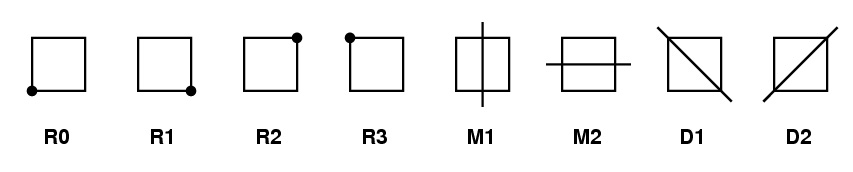
\includegraphics[width=14cm]{dih4}
\end{center}
}

\clearpage

Als je \'e\'en perfect vierkant hebt gevonden, kan je beweren dat je door te spiegelen en te roteren er nog $7$ andere hebt. Maar we zullen afspreken dat er van die acht perfecte vierkanten \'e\'en speciaal is, datgene dat zodanig gedraaid en gespiegeld wordt dat de vierkantjes binnenin het perfecte vierkant worden gerangschikt van groot naar klein. We beginnen linksboven en gaan naar rechts. Voor het grootste vierkant op een hoek heb je vier keuzes (\'e\'en keuze voor elke hoek). Kies nu zodanig dat het grootste vierkant linksboven komt te liggen. Rechts en onder dat vierkantje komen zeker opnieuw vierkantjes. Dus eigenlijk hebben we nu twee keuzen. We nemen deze keuze, zodanig dat het grootste van de twee keuzes rechts komt te liggen. We zullen zeggen dat de zeven andere perfecte vierkanten {\bf isomorf} zijn met het speciale geval, want er bestaat steeds een spiegeling of rotatie zodat we het perfecte vierkant in de speciale vorm krijgen.

\ask{Bepaal de bewerkingen (spiegelingen en/of rotaties) die uitgevoerd moeten worden op de volgende figuur om ze in de speciale vorm te krijgen:}

\answer{Hierop kan in \'e\'en keer de spiegeling $M1$ uitgevoerd worden. Alternatief kan ook gewerkt worden met rotaties gecombineerd met spiegelingen.}

\begin{center}
  \begin{tikzpicture}[scale=0.04,line cap=round,line join=round,>=triangle 45,x=1.0cm,y=1.0cm]
\clip(-5,-5) rectangle (115,115);
\filldraw[fill=black,fill opacity=0.05] (0,112.12) -- (33,112.12) -- (33,79.12) -- (0,79.12) -- cycle;
\filldraw[fill=black,fill opacity=0.05] (33,112.12) -- (70,112.12) -- (70,75.12) -- (33,75.12) -- cycle;
\filldraw[fill=black,fill opacity=0.05] (70,112.12) -- (112,112.12) -- (112,70.12) -- (70,70.12) -- cycle;
\filldraw[fill=black,fill opacity=0.05] (0,79.12) -- (29,79.12) -- (29,50.12) -- (0,50.12) -- cycle;
\filldraw[fill=black,fill opacity=0.05] (29,79.12) -- (33,79.12) -- (33,75.12) -- (29,75.12) -- cycle;
\filldraw[fill=black,fill opacity=0.05] (0,50.12) -- (50,50.12) -- (50,0.12) -- (0,0.12) -- cycle;
\filldraw[fill=black,fill opacity=0.05] (29,50.12) -- (29,75.12) -- (54,75.12) -- (54,50.12) -- cycle;
\filldraw[fill=black,fill opacity=0.05] (54,75.12) -- (70,75.12) -- (70,59.12) -- (54,59.12) -- cycle;
\filldraw[fill=black,fill opacity=0.05] (70,70.12) -- (88,70.12) -- (88,52.12) -- (70,52.12) -- cycle;
\filldraw[fill=black,fill opacity=0.05] (88,70.12) -- (112,70.12) -- (112,46.12) -- (88,46.12) -- cycle;
\filldraw[fill=black,fill opacity=0.05] (54,59.12) -- (63,59.12) -- (63,50.12) -- (54,50.12) -- cycle;
\filldraw[fill=black,fill opacity=0.05] (63,59.12) -- (70,59.12) -- (70,52.12) -- (63,52.12) -- cycle;
\filldraw[fill=black,fill opacity=0.05] (63,52.12) -- (65,52.12) -- (65,50.12) -- (63,50.12) -- cycle;
\filldraw[fill=black,fill opacity=0.05] (82,52.12) -- (88,52.12) -- (88,46.12) -- (82,46.12) -- cycle;
\filldraw[fill=black,fill opacity=0.05] (65,52.12) -- (82,52.12) -- (82,35.12) -- (65,35.12) -- cycle;
\filldraw[fill=black,fill opacity=0.05] (50,50.12) -- (65,50.12) -- (65,35.12) -- (50,35.12) -- cycle;
\filldraw[fill=black,fill opacity=0.05] (50,0.12) -- (50,35.12) -- (85,35.12) -- (85,0.12) -- cycle;
\filldraw[fill=black,fill opacity=0.05] (82,35.12) -- (82,46.12) -- (93,46.12) -- (93,35.12) -- cycle;
\filldraw[fill=black,fill opacity=0.05] (93,46.12) -- (112,46.12) -- (112,27.12) -- (93,27.12) -- cycle;
\filldraw[fill=black,fill opacity=0.05] (85,35.12) -- (93,35.12) -- (93,27.12) -- (85,27.12) -- cycle;
\filldraw[fill=black,fill opacity=0.05] (85,27.12) -- (112,27.12) -- (112,0.12) -- (85,0.12) -- cycle;
\draw (-0.01,111.81)-- (-0.01,0.32);
\draw (-0.01,0.32)-- (-0.01,111.81);
\end{tikzpicture}

\end{center}

Dit lukt dus niet om meerdere perfecte vierkanten te vinden. Laten we nu eens iets anders proberen. Als we het perfecte vierkant zodanig zouden vergroten dat er plaats is in het kleinste vierkantje om het originele perfecte vierkant erin te passen. Dan vinden we toch al twee perfecte vierkanten!

\ask{Met welke factor moet het perfecte vierkant van orde 21 vergroot worden zodat een perfect vierkant van orde 21 past in het kleinste vierkantje?}

\answer[5]{Het kleinste vierkantje heeft grootte $2$ en het totale vierkant heeft grootte $50+35+27=112$. Als we dus alle lengtes vermenigvuldigen met $\frac{112}{2}=56$ dan past in het nieuwe kleinste vierkantje het originele perfecte vierkant!}

Nu vinden we dus al een extra perfect vierkant aan de hand van ons oorspronkelijk perfect vierkant. Deze procedure kan herhaald worden om dan een derde, vierde, vijfde, \ldots perfecte vierkant te vinden. Deze procedure kan ook in de andere richting herhaald worden. Dus ook het kleine vierkantje kan gevuld worden met hetzelfde perfecte vierkant. Dan moeten natuurlijk wel alle groottes gedeeld worden. Als we nu in beide richtingen deze procedure oneindig lang herhalen dan krijgen we een meetkundige figuur die zelfgelijkend is. Zulk een figuur noemen we een {\bf fractaal}.

\subsubsection{Eigenschap over het kleinste vierkant in een perfect vierkant}

We hebben al gezien dat het kleinste vierkant in een perfect vierkant speciaal is. We kunnen het gebruiken om nog meer perfecte vierkanten te construeren. Het is ook opmerkelijk dat het kleinste vierkant nooit aan de rand van het perfecte vierkant kan liggen.

\ask{Probeer eens om wel het kleinste vierkant op de zijkant te plaatsen. Hoeveel vierkanten zullen er dan nog rond het kleinste vierkantje zitten? En wat weten we over deze vierkanten rond het kleinste vierkant?}

\answer[3cm]{Dit lukt niet. Rond het kleinste vierkant moeten dan nog 3 andere vierkantjes komen want \'e\'en zijde ligt aan de rand van het perfecte vierkant. Die drie andere vierkanten zijn allemaal groter dan het kleinste vierkant, dus \'e\'en van die vierkanten zal over de rand komen te liggen, waardoor het geen perfect vierkant meer is.}

Hier geef je een bewijs uit het ongerijmde. Je veronderstelt dat je wel iets kan. Bijvoorbeeld het kleinste vierkant op de rand van een perfect vierkant leggen. Dan toon je aan dat je tot een tegenstrijdigheid komt. Dus \'e\'en van de vierkantjes die rond het kleinste vierkant ligt zal over de rand komen te liggen. Het perfecte vierkant is geen perfect vierkant! Hierdoor weet je dat de veronderstelling niet kan. Dus dat het kleinste vierkantje niet op de rand kan liggen. Zie dit visueel in Figuur \ref{fig:pv_kleinstevierkant}.

\begin{figure}
\begin{center}
  \definecolor{cccccc}{rgb}{0.6,0.6,0.6}
\begin{tikzpicture}[scale=0.3, line cap=round,line join=round,>=triangle 45,x=1.0cm,y=1.0cm]
\clip(45,32) rectangle (75,61);
\draw [line width=1.2pt, color=cccccc] (65,32) -- (65,61);
\filldraw[line width=1.2pt,fill=black,fill opacity=0.1] (54,59.12) -- (63,59.12) -- (63,50.12) -- (54,50.12) -- cycle;
\filldraw[line width=1.2pt,fill=black,fill opacity=0.1] (63,59.12) -- (70,59.12) -- (70,52.12) -- (63,52.12) -- cycle;
\filldraw[line width=1.2pt,fill=black,fill opacity=0.15] (63,52.12) -- (65,52.12) -- (65,50.12) -- (63,50.12) -- cycle;
\filldraw[line width=1.2pt,fill=black,fill opacity=0.1] (50,50.12) -- (65,50.12) -- (65,35.12) -- (50,35.12) -- cycle;
\end{tikzpicture}

\end{center}
\caption{Het kleinste vierkant in een perfect vierkant kan niet op de rand liggen.}
\label{fig:pv_kleinstevierkant}
\end{figure}

\subsection{Perfecte kubussen}

In de wiskunde veralgemenen we graag onze resultaten naar alle dimensies. In de les van de perfecte vierkanten hebben we steeds in een vlak gewerkt. Daarbinnen hebben we dan in een vierkant gewerkt. Dit is het tweedimensionale geval. Er bestaat dus een simpeler \'e\'endimensionale geval. Hier wordt dan op een rechte een lijnstuk genomen.% Dit lijnstuk moet dan gevuld worden met allemaal lijnstukken met verschillende natuurlijke lengtes.

\task{Geef zelf een definitie voor een perfect lijnstuk analoog als voor een perfect vierkant.}

\answer[3cm]{Een lijnstuk is een {\bf perfect lijnstuk} als het volledig gevuld wordt met kleinere lijnstukken die allemaal een andere lengte hebben.}

\ask{Toon aan hoe je een perfect lijnstuk kunt construeren met de kleinere lijnstukken van lengte $1$, $2$ en $3$. Waarom zullen we hier weinig nieuwe wiskunde in ontdekken?}

\answer[3cm]{Plaats de drie lijnstukken achter elkaar. Dit geeft dan een nieuw lijnstuk dat aan de voorgaande definitie van perfect lijnstuk voldoet. Hadden we de drie lijnstukken in een andere volgorde geplaatst, dan was de constructie van een perfect lijnstuk ook gelukt. Het is steeds mogelijk om perfecte lijnstukken te vinden zonder te puzzelen, voeg gewoon een nieuw lijnstuk met nieuwe lengte toe en we hebben een nieuw perfect lijnstuk.}

\teacher{Het is ook belangrijk op te merken dat er in 1-dimensie geen analogon is voor een vierkant. In drie dimensies heb je wel kubussen. Een lijnstuk kan eerder vergeleken worden met een rechthoek in 2 dimensies of een balk in 3 dimensies.}

Als dan het 1-dimensionale geval weinig uitdagend is, dan is het 3-dimensionale geval het misschien wel. Als we een kubus krijgen, is het dan mogelijk om deze kubus op te splitsen in een eindig aantal kleinere kubussen waarvan er geen twee dezelfde grootte hebben? Het antwoord op deze vraag blijkt neen te zijn!

Het is onmogelijk om dit te bewijzen door alle mogelijke groottes van kubussen te overlopen en te controleren dat het nooit lukt. Simpelweg omdat we dan oneindig veel kubussen zouden moeten controleren. We moeten dus een argument vinden waarom het dan niet lukt. Ook hier zal een bewijs uit het ongerijmde ons dat argument leveren. We moeten dus beginnen met het tegendeel te veronderstellen.

\ask{Wat is het tegendeel van hetgeen we zullen bewijzen?}

\answer[2cm]{We zullen bewijzen dat er geen kubus bestaat die opgesplitst kan worden in een eindig aantal kleinere kubussen waarvan er geen twee dezelfde grootte hebben. Het tegendeel is dan dat er wel zulk een kubus bestaat.}

\ask{Veronderstel nu dat er wel een kubus bestaat die opgesplitst kan worden in een eindig aantal kleinere kubussen waarvan er geen twee dezelfde grootte hebben. Hoe ziet het onderste vlak van deze kubus er dan uit?}

\answer[2cm]{Dit moet dan een perfect vierkant zijn.}

Als we dan enkel de onderste kubussen laten staan, dan krijgen we in het vlak een vierkant met allemaal kubussen van verschillende grootte. Ergens op dat vlak moet dan een kleinste kubus liggen.

\ask{Wat weten we over de ligging van deze kleinste kubus?}

\answer[3cm]{Deze kleinste kubus kan niet aan de zijkant liggen, want alle kubussen liggen op een perfect vierkant en we weten dat het kleinste vierkant van een perfect vierkant niet aan de zijkant kan liggen.}

\ask{Ten opzichte van deze kleinste kubus zijn al zijn buren grotere kubussen. Wat wil dit nu zeggen voor de kubus die boven deze kleinste kubus moet komen?}

\answer[4cm]{Het is niet toegestaan om opnieuw een kubus van deze grootte te gebruiken, een grotere kubus zal niet passen, dus moeten er verschillende kleinere kubussen boven deze kleinste kubus komen.}

Kleinere kubussen moeten volledig het vlak boven deze kleinste kubus opvullen. Dit wil zeggen dat dit vlak van de kubus een perfect vierkant moet zijn gevuld met kubussen. We kunnen nu de zelfde argumentatie gebruiken op de kleinste kubus van dit vlak. Zo moeten we steeds verder gaan. Omdat de volumes van kubussen groter dan nul moeten zijn zal dit proces ooit stoppen. We kunnen niet zowel steeds verder gaan en ooit stoppen, we hebben dus een tegenstrijdigheid!

%\question{Dit argument wordt in het Engels "Infinite descent" genoemd. Wat is de correcte vertaling naar het nederlands? -> Oneindig dalende rij}







